\subsection{Dati e risultati}

\paragraph{Slew rate}

La prima parte dell'esperienza era centrata sulla misura dello slew rate
dell'amplificatore operazionale. Lo slew rate è il tasso di cambiamento massimo
della tensione di uscita per unità di tempo. Anche se idealmente un operazionale
risponde istantaneamente ai cambiamenti in ingresso, in realtà impiega del tempo
ad adattare la tensione di uscita, soprattutto perché contiene dei condensatori.

Per misurare lo slew rate del nostro operazionale, abbiamo montato il circuito
\ref{fig:slew_circ3}, che è il circuito standard per fare queste misure ed
è riportato nel manuale del costruttore dell'opamp. Il circuito è semplice ed è pensato
per una misura diretta. Il ramo di feedback serve per fare un amplificatore 
con guadagno unitario (un follower), mentre resistenza e capacità servono per polarizzare
l'operazionale e per tagliare le frequenze alte (i rimbalzi che si hanno ai bordi delle onde quadre).

\begin{figure}[t!]
    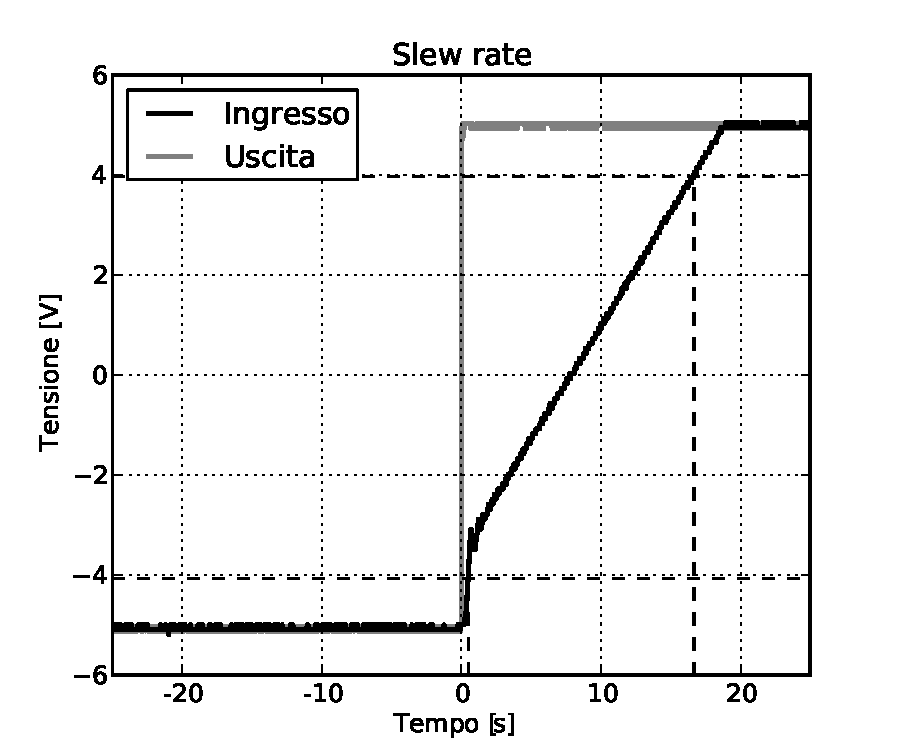
\includegraphics[width=\columnwidth]{figure/slew_graph1.pdf}
    \caption{La figura mostra il comportamento dell'operazionale ad un brusco cambiamento della tensione
        differenziale in ingresso. Il circuito realizzato (il \ref{fig:slew_circ3}) è un emitter follower
        e dovrebbe copiare il segnale in ingresso all'uscita. Invece, a causa del fatto che lo slew rate
        dell'operazionale è finito, la tensione impiega circa 20 $\mu$s a passare da -5 V a 5 V.}
    \label{fig:slew_graph3}
\end{figure}

Per la misura si fornisce in input un'onda quadra generata con il generatore
di funzioni d'onda (Che ha uno slew rate molto alto che fa si che il suo output sia
molto vicino ad un onda quadra. Abbiamo misurato uno slew rate di circa 500 V/$\mu$s per
il nostro generatore.) e si misura $V\ped{out}$, che è un trapezio a causa appunto dello
slew rate finito dell'operazionale. La figura  \ref{fig:slew_graph3} mostra un esempio
di quello che succede dando in ingresso un onda quadra.
Per convenzione, si misura il tempo impiegato
dalla tensione per salire dal 10\% al 90\% della tensione massima dello scalino.
Lo slew rate è calcolabile così:

\begin{equation}
    S = \frac{V\ped{90\%} - V\ped{10\%}}{t\ped{90\%} - t\ped{90\%}}
\end{equation}

Nelle nostre misure abbiamo utilizzato un onda quadra di 10 Vpp a 1 kHz.
Misurando lo slew rate sia in salita che in discesa, e abbiamo ottenuto
due valori diversi

\begin{equation}
    S\ped{salita} = 0.498 \pm 0.004 \; \text{V/$\mu$s}
\end{equation}
\begin{equation}
    S\ped{discesa} = -0.353 \pm 0.003 \; \text{V/$\mu$s}
\end{equation}

Il valore in salita è vicinissimo al dato specificato dal produttore: 0.5 V/$\mu$s.
Il dato in discesa è minore circa del 30\% rispetto a quello in salita.

Lo slew rate ha implicazioni piuttosto pesanti ad alte frequenze di funzionamento del circuito.
Infatti se all'amplificatore operazionale è dato in input un segnale che varia in maniera molto
veloce (un segnale periodico ad alta frequenza), ad un certo punto l'amplificatore non riuscirà
più a ''star dietro``, per così dire, al segnale, e inizierà a deformarlo. Per verificare questo
comportamento, abbiamo usato lo stesso circuito di prima, ma il generatore di forme d'onda è
stato impostato per fornire un'onda sinusoidale 10 Vpp di divese frequenze. Variando la frequenza
abbiamo notato che il segnale inizia ad essere deformato a circa 13 kHz (solo in discesa ovviamente,
poiché lo slew rate è minore). In figura \ref{fig:slew_signal3} sono mostrati input e output
alla frequenza di 20 kHz. La deformazione del segnale è evidente sia in salita che in discesa ed è
pure abbastanza seria, nonostante la frequenza non sia poi così alta (è grande l'ampiezza del segnale).

\begin{figure}[t]
    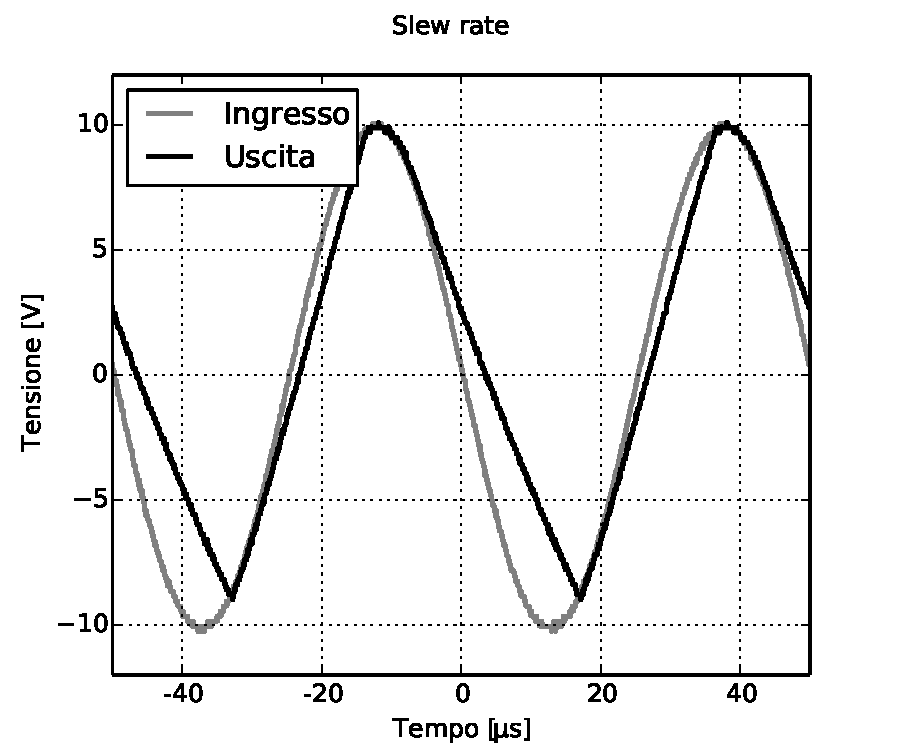
\includegraphics[width=\columnwidth]{figure/slew_signal3.pdf}
    \caption{La figura mostra il comportamento dell'operazionale ad un brusco cambiamento della tensione
        differenziale in ingresso. Il circuito realizzato (il \ref{fig:slew_circ3}) è un emitter follower
        e dovrebbe copiare il segnale in ingresso all'uscita. Invece, a causa del fatto che lo slew rate
        dell'operazionale è finito, la tensione impiega circa 20 $\mu$s a passare da -5 V a 5 V.}
    \label{fig:slew_signal3}
\end{figure}

\paragraph{Corrente massima}

In questo paragrafo ci proponiamo di misurare la corrente massima che il nostro amplificatore
riesce a fornire dall'uscita. Per la misura ci siamo serviti del circuito \ref{fig:max_curr_circ3}.
Il circuito è semplicissimo: è simile al precedente, ma tra l'uscita e terra è presente solo una resistenza
molto piccola (100 \si{\ohm}) in modo che la tensione $v\ped{out}$ non sia determinata dalla tensione
in ingresso, bensì dalla massima corrente che l'amplificatore riesce a fornire. Misurando $V\ped{out}$.
si ricava banalmente la corrente dalla legge di Ohm, assumendo che la corrente assorbita dall'ingresso
invertente sia trascurabile.

Abbiamo fornito in input un'onda triangolare di 10 Vpp a 1 kHz. L'uscita registrata è stata un'andamento,
sempre triangolare, di 2.7 V da picco a picco. Dividendo a metà (cioè prendendo la massima tensione che $V\ped{out}$
assume, nell'altra metà dell'onda la corrente scorre semplicemente al rovescio) e usando la legge di Ohm
si ottiene $I\ped{max} = 13.5 \pm 0.7$ mA. Il range tipico riportato sul manuale è 10-20 mA.

\paragraph{Banda passante}